\documentclass[aspectratio=169]{beamer}
\usetheme{Madrid}
\usecolortheme{default}
\setbeamertemplate{navigation symbols}{}
\usepackage[T1]{fontenc}
\usepackage[utf8]{inputenc}
\usepackage{lmodern}
\usepackage{graphicx}
\usepackage{booktabs}
\usepackage{array}
\graphicspath{{../assets/figures/}{../../reports/publication/}}

\title{ORIUS: Universal-First Monograph Defense}
\subtitle{Physical AI Safety under Degraded Observation}
\author{Pratik Niroula}
\date{April 2026}

\begin{document}

\begin{frame}
  \titlepage
\end{frame}

\begin{frame}{Thesis Claim}
  \begin{itemize}
    \item ORIUS is a universal runtime safety layer for physical AI under degraded observation.
    \item The monograph now reads as one argument: hazard $\rightarrow$ architecture $\rightarrow$ theory $\rightarrow$ domains $\rightarrow$ governed closure lane.
    \item The book is universal-first in structure and three-domain in evidence.
    \item Battery remains the reference witness; healthcare and bounded AV are defended rows.
  \end{itemize}
\end{frame}

\begin{frame}{Book Structure}
  \begin{enumerate}
    \item Why Physical AI Needs a Safety Layer
    \item ORIUS Architecture
    \item Theory
    \item Domain Chapters
    \item Universality, Limits, and Societal Program
    \item Appendices: proofs, protocol cards, review dossier, artifact index
  \end{enumerate}
\end{frame}

\begin{frame}{Theory to Runtime to Domain Flow}
  \centering
  
\includegraphics[width=0.96\textwidth]{fig_orius_theory_runtime_domain_flow.png}
\end{frame}

\begin{frame}{Universal Runtime Architecture}
  \centering
  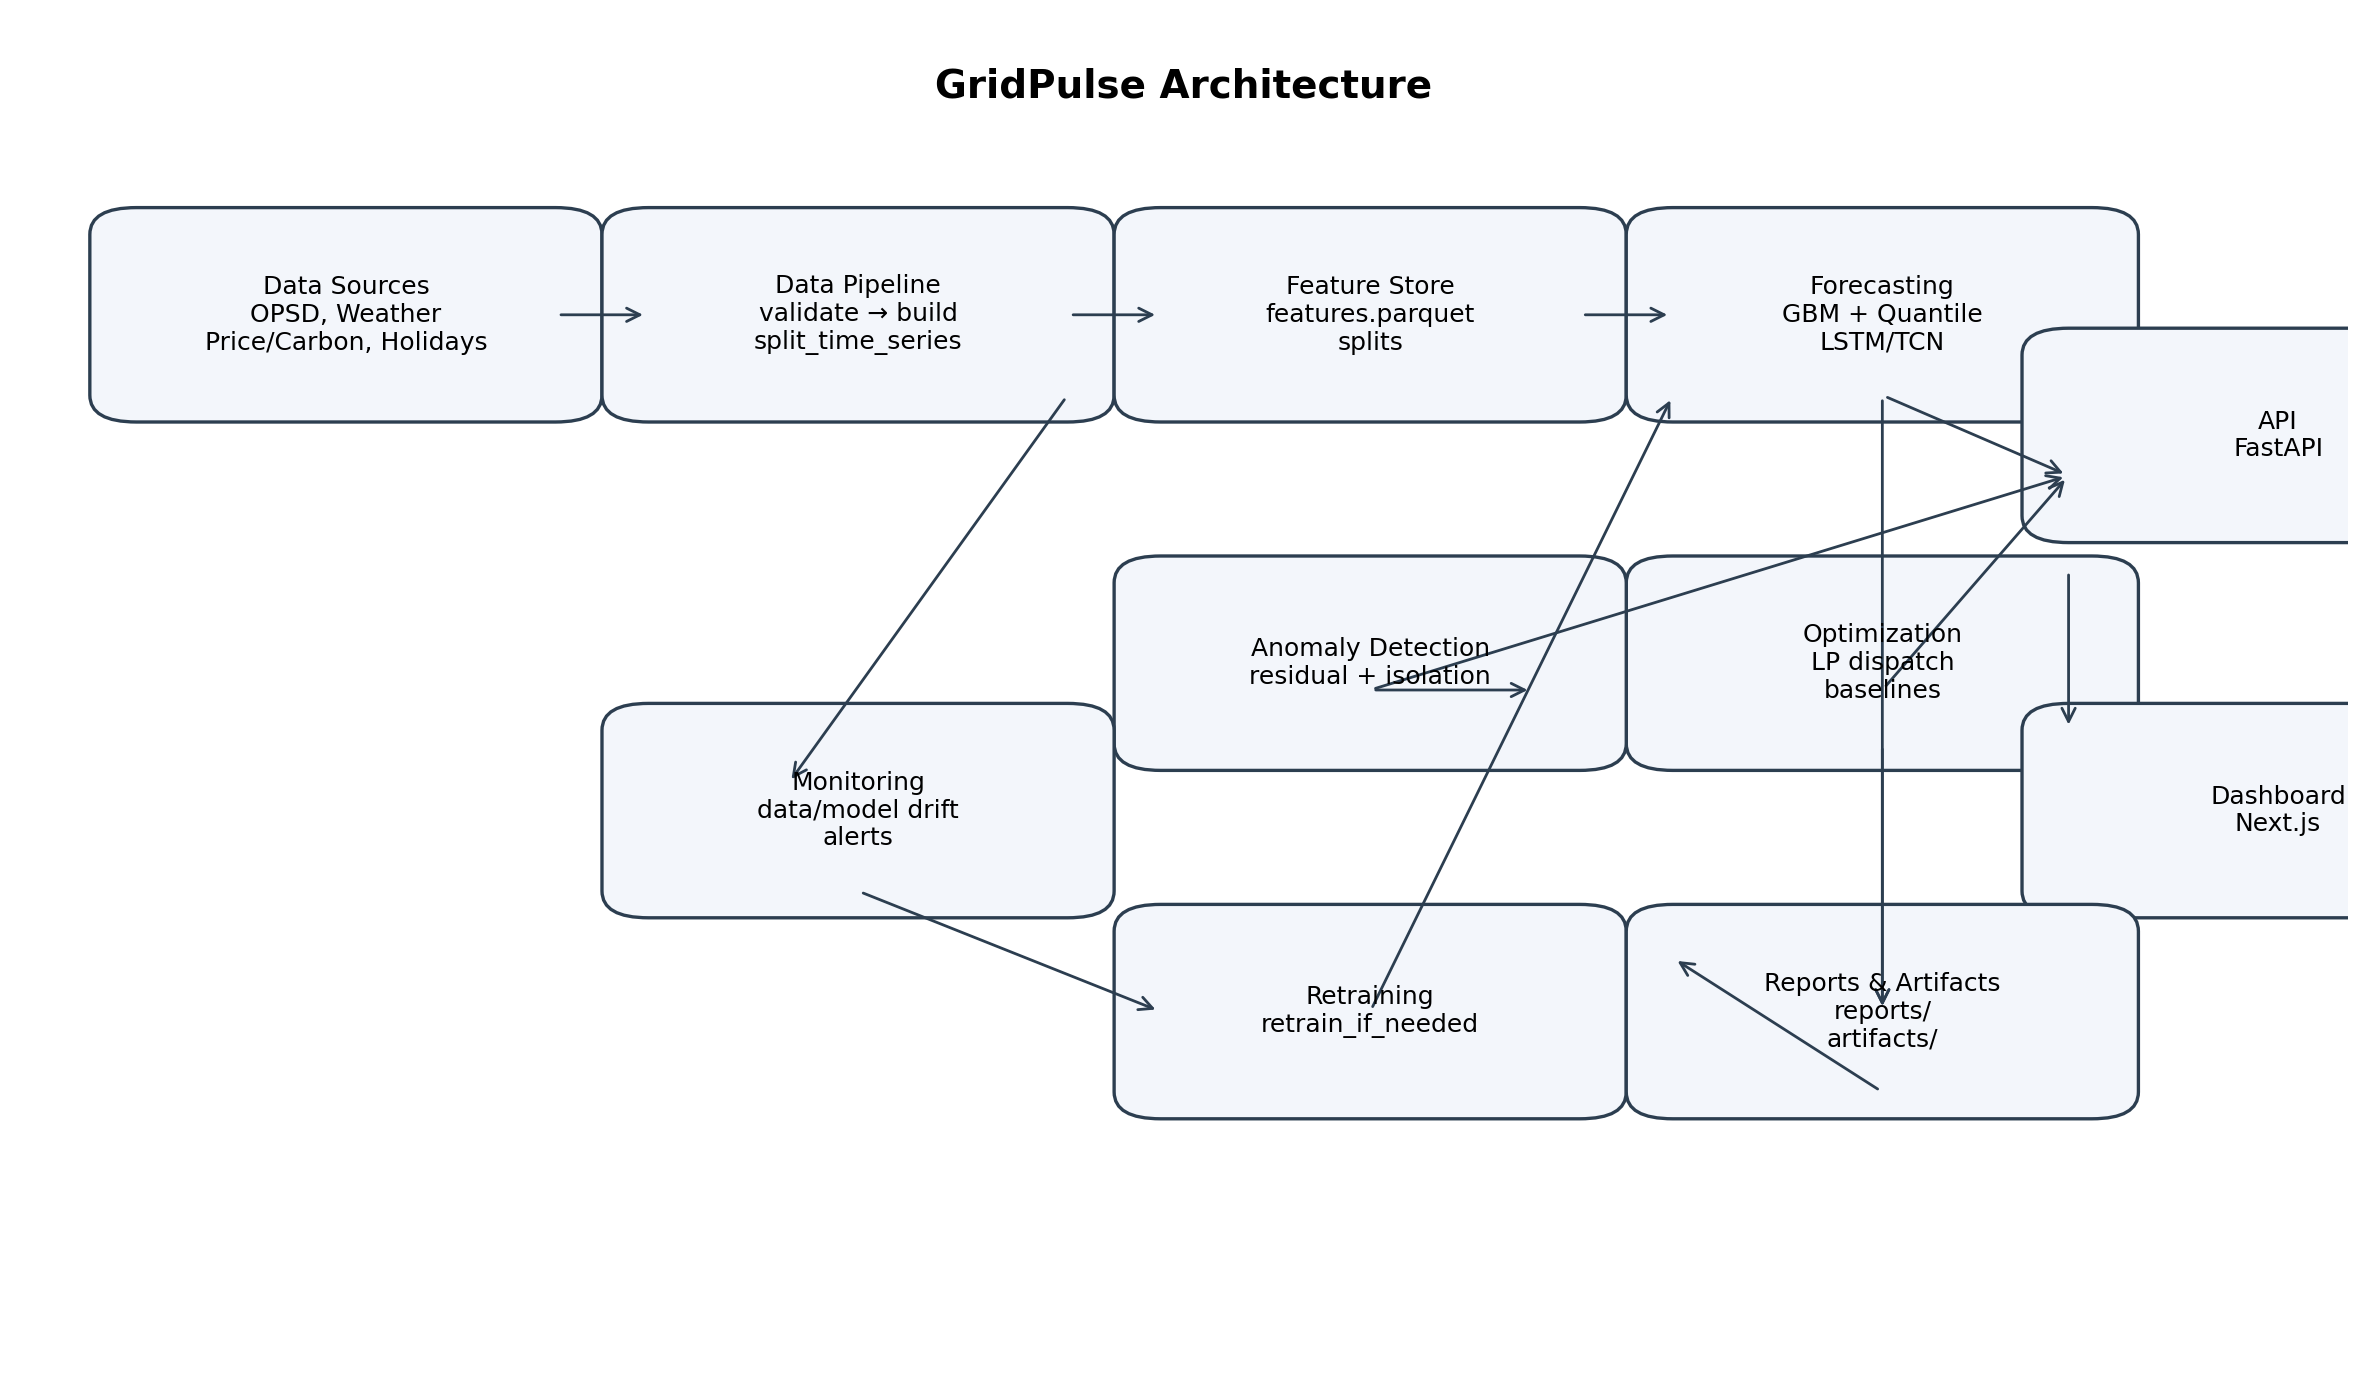
\includegraphics[width=0.94\textwidth]{fig01_architecture.png}
\end{frame}

\begin{frame}{Program Spine}
  \centering
  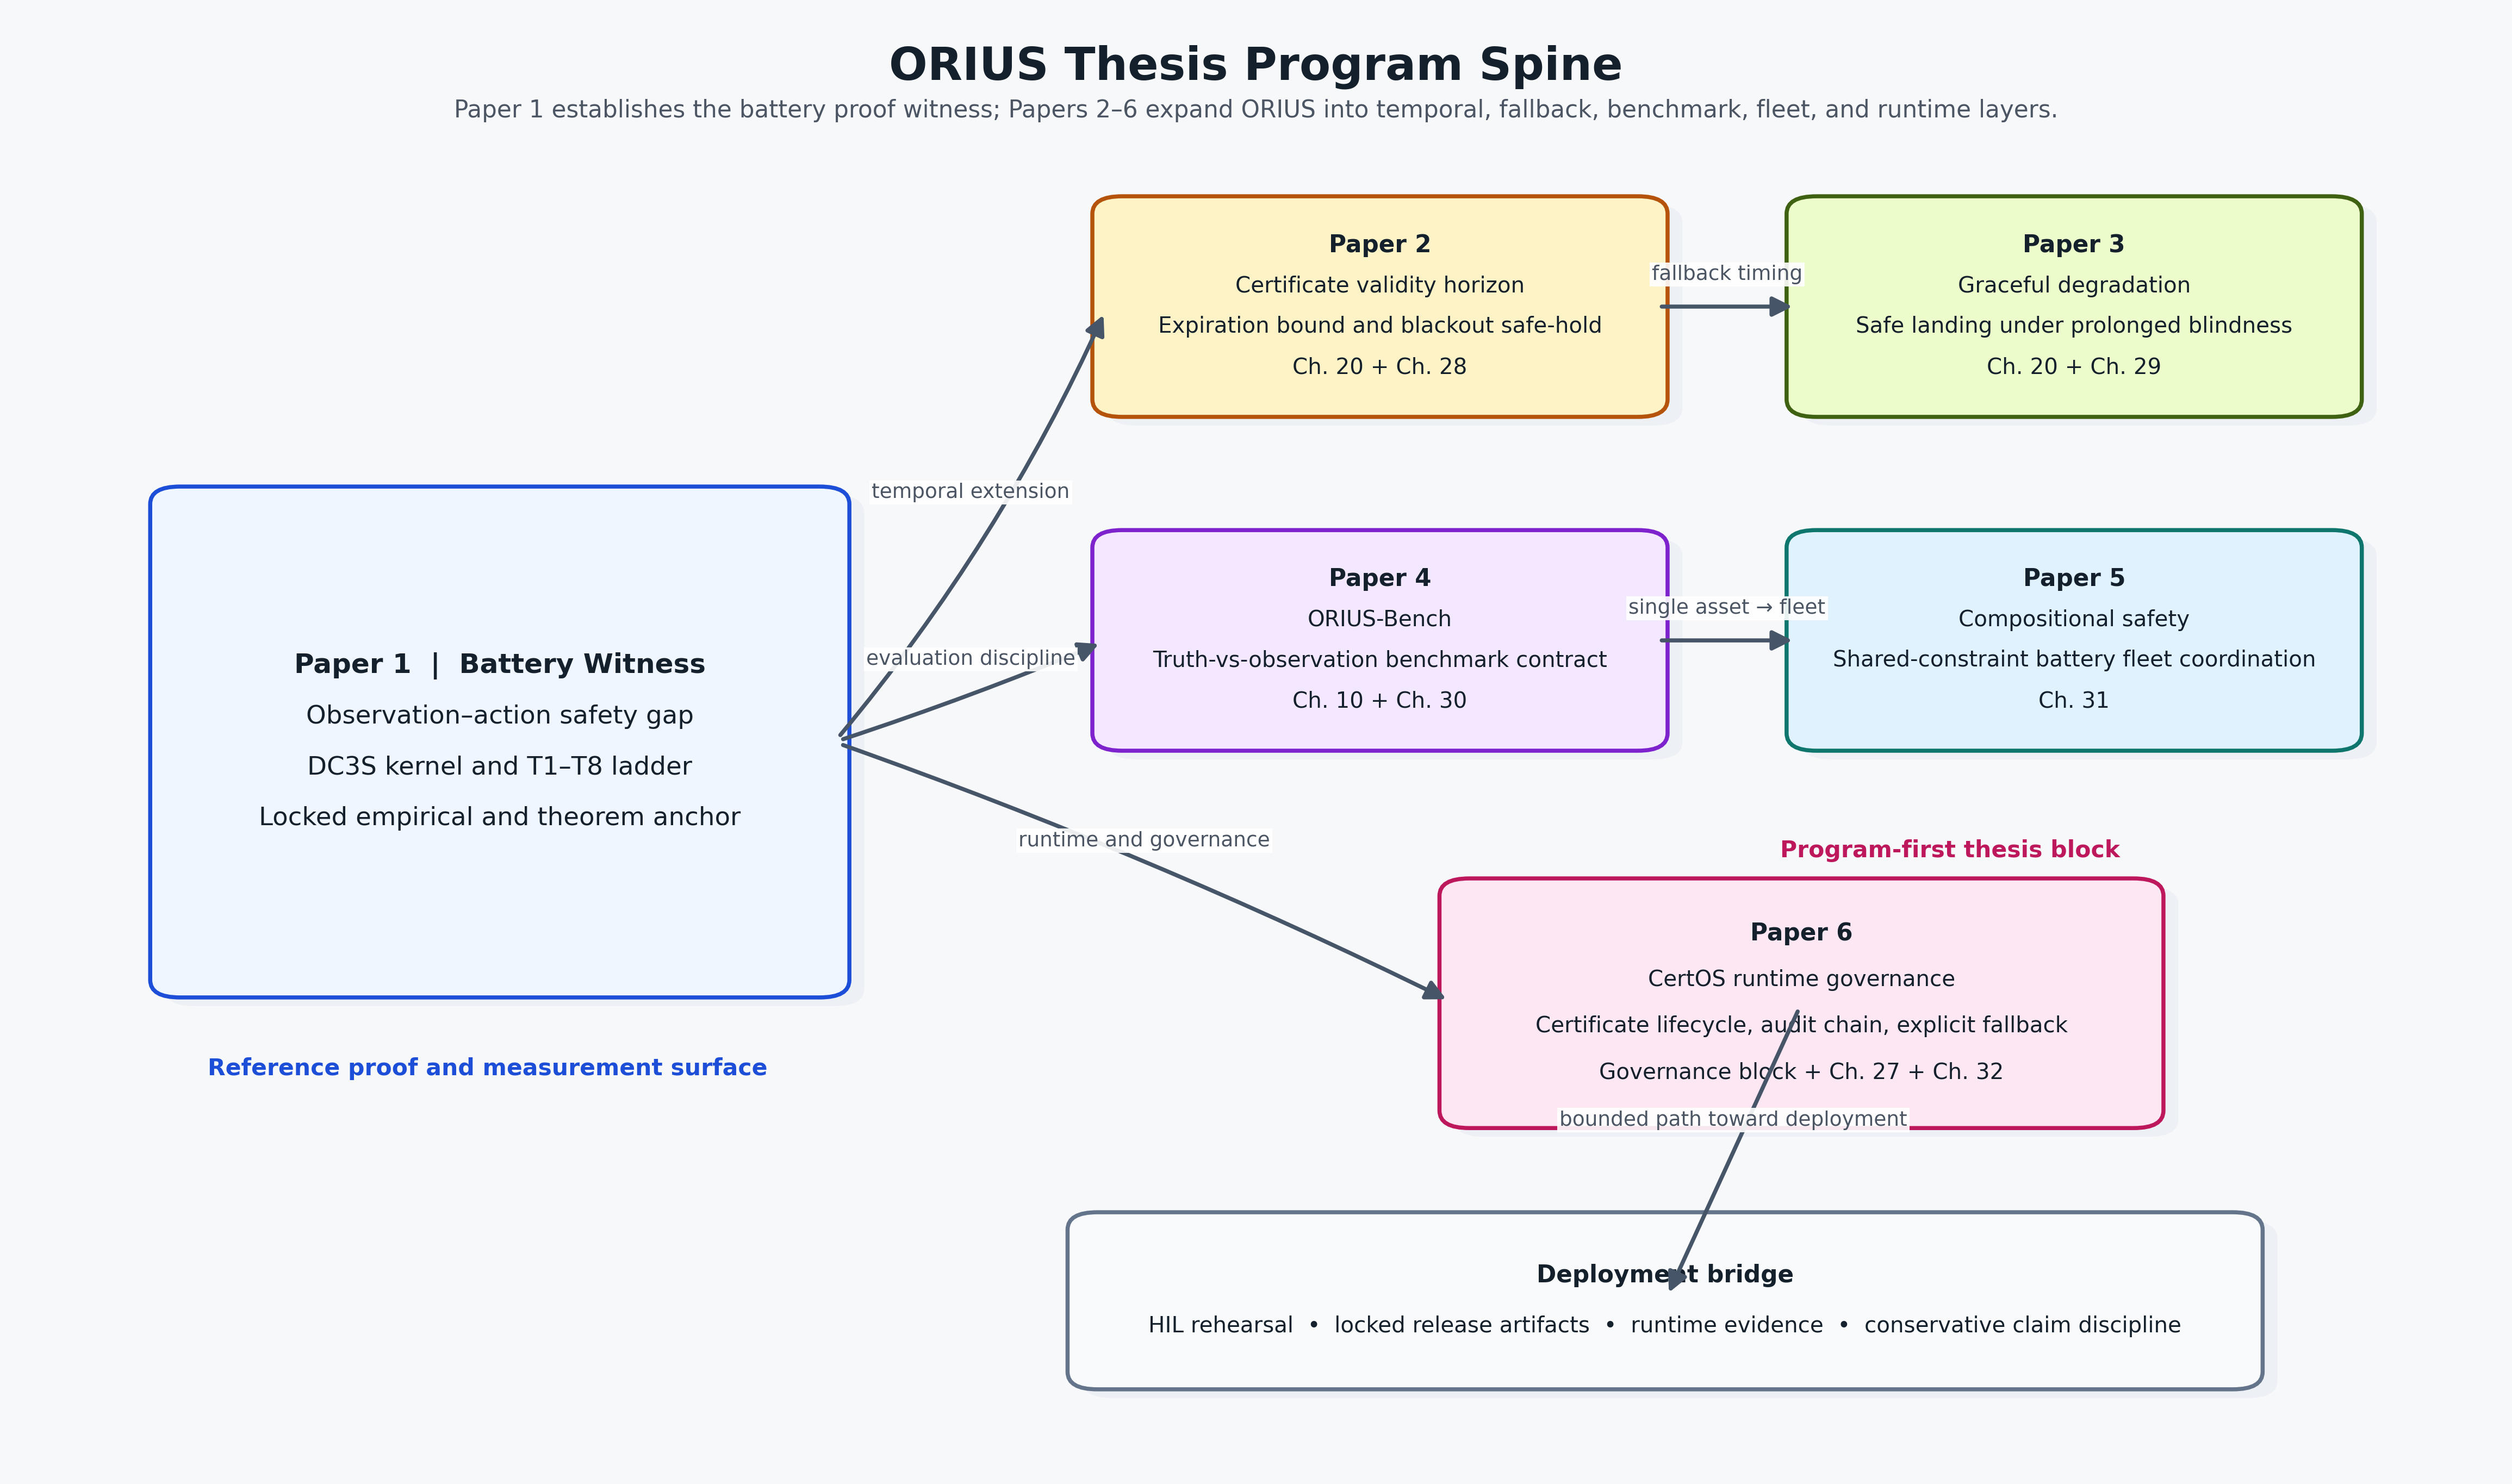
\includegraphics[width=0.88\textwidth]{fig46_orius_program_spine.png}
\end{frame}

\begin{frame}{Current Closure Matrix}
  \centering
  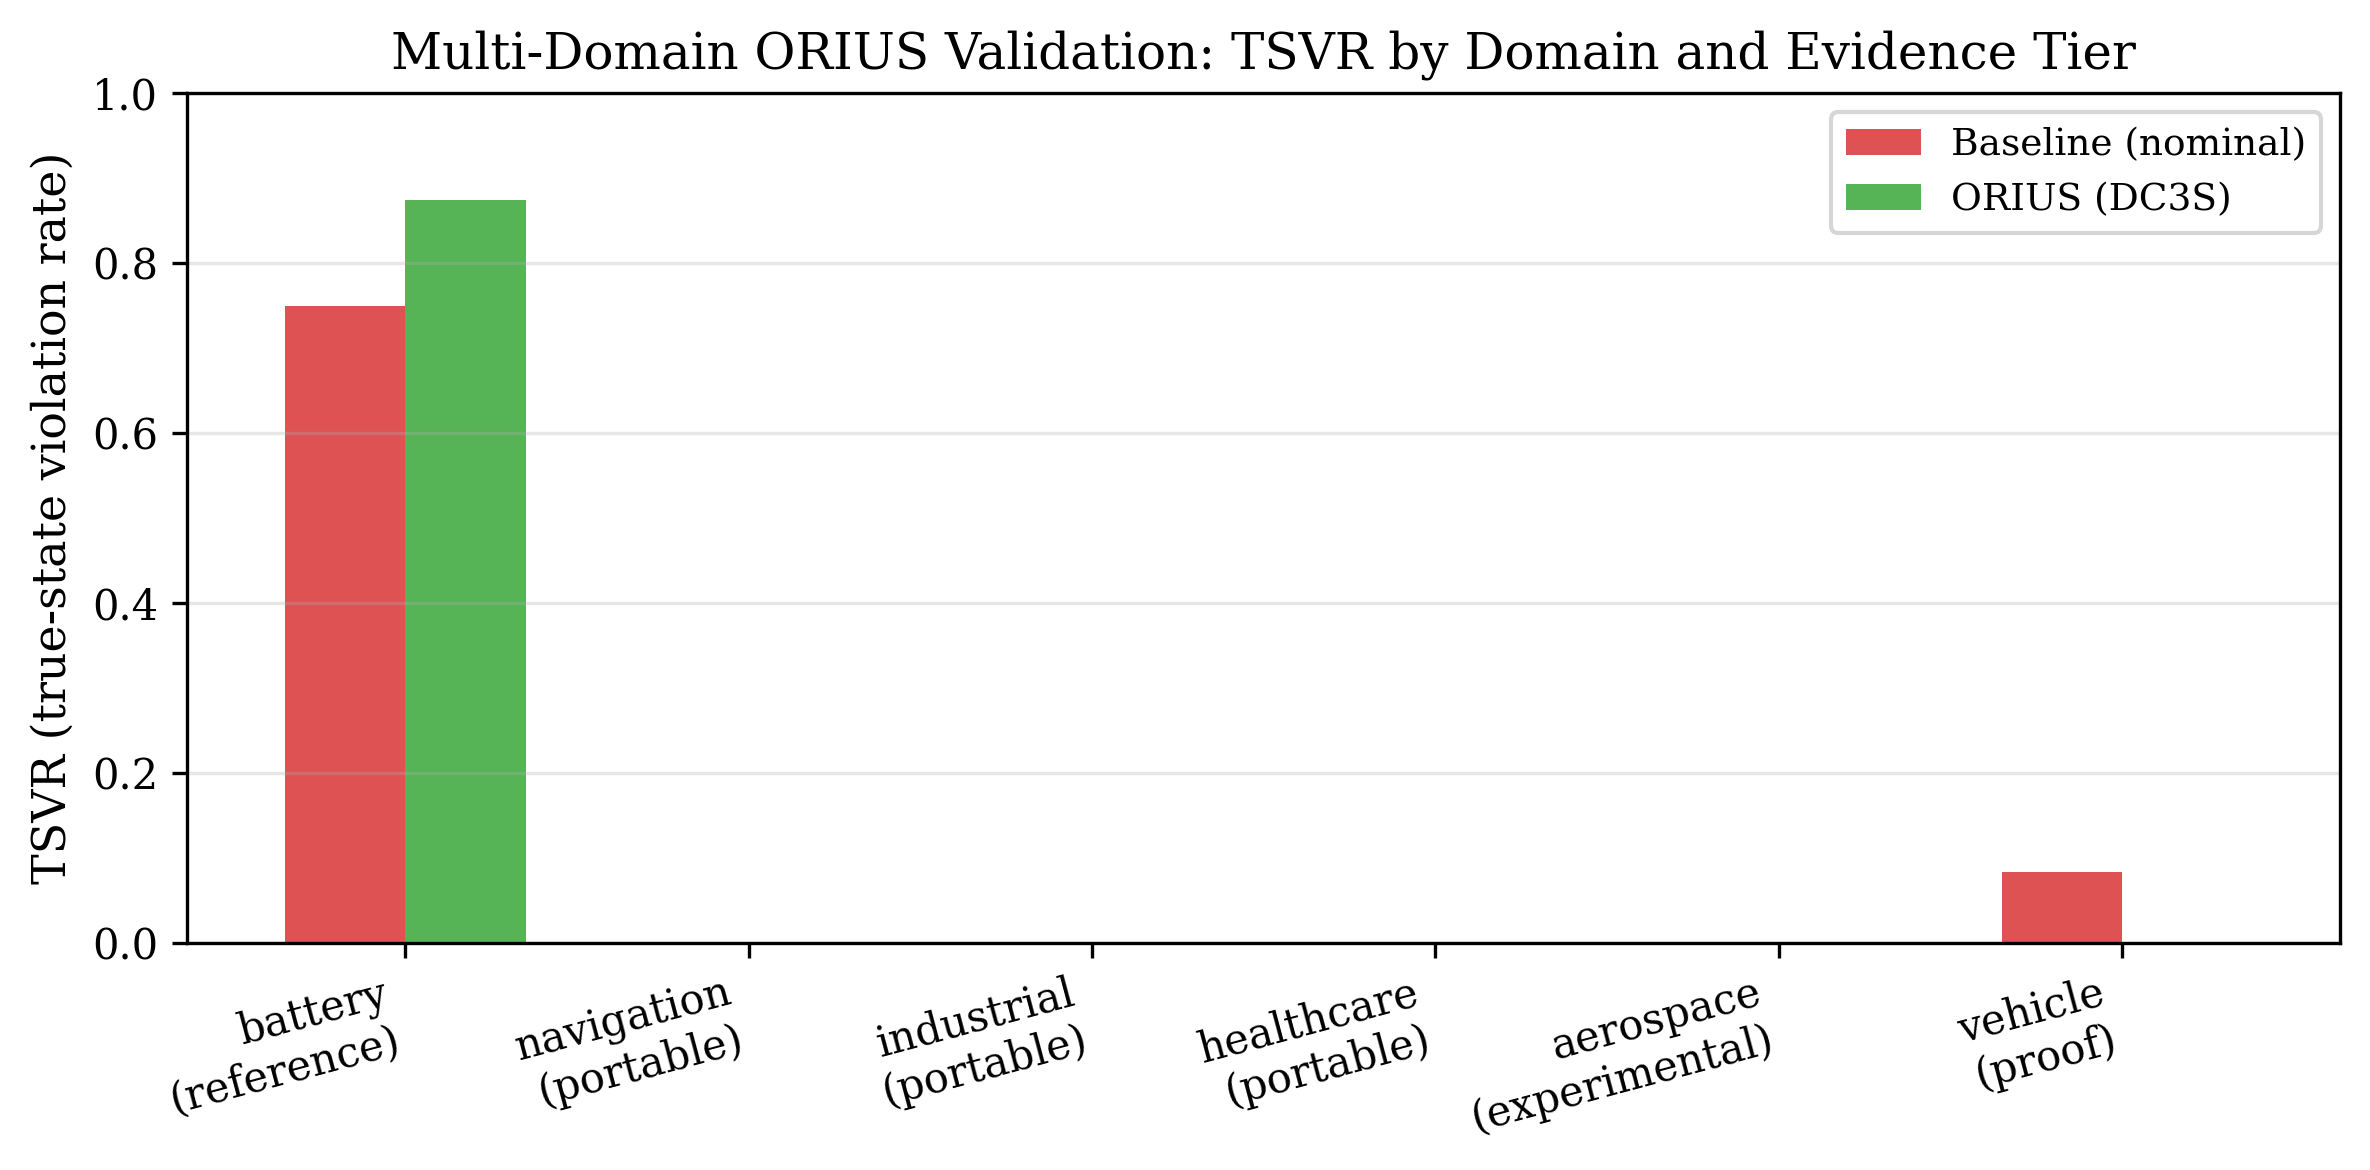
\includegraphics[width=\textwidth]{fig_multi_domain_validation.png}
\end{frame}

\begin{frame}{Current Domain Status}
  \begin{tabular}{>{\raggedright\arraybackslash}p{0.24\textwidth} >{\raggedright\arraybackslash}p{0.22\textwidth} >{\raggedright\arraybackslash}p{0.44\textwidth}}
    \toprule
    Domain & Current Tier & Current Truth \\
    \midrule
    Battery & Reference & Full theorem-to-artifact witness \\
    Autonomous vehicles & Proof-validated & Bounded TTC + predictive-entry-barrier contract cleared \\
    Healthcare & Proof-validated & Bounded monitoring/intervention row \\
    \bottomrule
  \end{tabular}
\end{frame}

\begin{frame}{Bounded Universality}
  \begin{itemize}
    \item The book does not blur universal architecture with equal-domain closure.
    \item Universal claim: one kernel, one adapter contract, one benchmark/governance stack.
    \item Bounded claim: promotion still depends on row-specific replay, soundness, fallback, and artifact closure.
    \item This makes the monograph stronger, not weaker: it is ambitious in architecture and disciplined in evidence.
  \end{itemize}
\end{frame}

\begin{frame}{Composition and Governance}
  \begin{itemize}
    \item Composition and CertOS are integrated as bounded universal layers, not separate reader-facing artifacts.
    \item Shared-constraint composition is treated as a bounded coordination layer inside the framework.
    \item Certificate lifecycle, audit, fallback, and recovery sit inside the runtime governance layer.
    \item Cross-domain evaluation exists where adapters support it and stays gated elsewhere.
  \end{itemize}
\end{frame}

\begin{frame}{R1 Review Program}
  \begin{itemize}
    \item Five reviewer personas: controls, CPS/systems, uncertainty/calibration, deployment safety, dissertation coherence.
    \item Three waves: outline, full draft, near-final PDF.
    \item Deliverables: scorecards, global gap matrix, remediation report, review dossier PDF.
    \item Review conclusion: structure is now R1-grade for the active three-domain program.
  \end{itemize}
\end{frame}

\begin{frame}{What Is Ready Now}
  \begin{itemize}
    \item 450+ page universal-first monograph PDF
    \item 183-reference bibliography
    \item three-domain closure artifact and review dossier
    \item explicit claim boundaries for the active Battery, AV, and Healthcare rows
  \end{itemize}
\end{frame}

\begin{frame}{Takeaway}
  \begin{block}{Bottom line}
    ORIUS is now packaged as a serious universal-first monograph with a clean R1-style review surface. The strongest honest submission claim is a universal physical-AI safety framework defended on Battery, AV, and Healthcare with an explicit bounded evidence surface.
  \end{block}
\end{frame}

\end{document}
